%/*****************************************************************************
% * WindNinja Tutorial 4
%/*****************************************************************************

\documentclass[12pt]{article}
\usepackage{float}
\usepackage{graphicx}
\usepackage{longtable}
\usepackage[margin=1in]{geometry}
\usepackage[table,x11names]{xcolor}

\graphicspath{{imgs/}}

\usepackage[utf8]{inputenc}
\usepackage[english]{babel}
\usepackage[parfill]{parskip}
\usepackage{datetime}
\usepackage{hyperref}
\hypersetup{
	colorlinks=true,
	urlcolor=blue,
  }
\urlstyle{same}
\usepackage{subcaption} 
\usepackage{dirtytalk}
\usepackage{multirow}
\usepackage{booktabs}

\usepackage{pdflscape}

\usepackage{adjustbox}

\usepackage{fancyhdr}
\pagestyle{fancy}
\fancyhf{}
\rhead{WindNinja Tutorial 4: Weather Model Initialization}
\cfoot{\thepage}

\newcommand\vn{3.8.0}

\begin{document}
\begin{titlepage}
    \centering
    {\Huge
       WindNinja Tutorial 4: Weather Model Initialization
    }    
    \vfill
    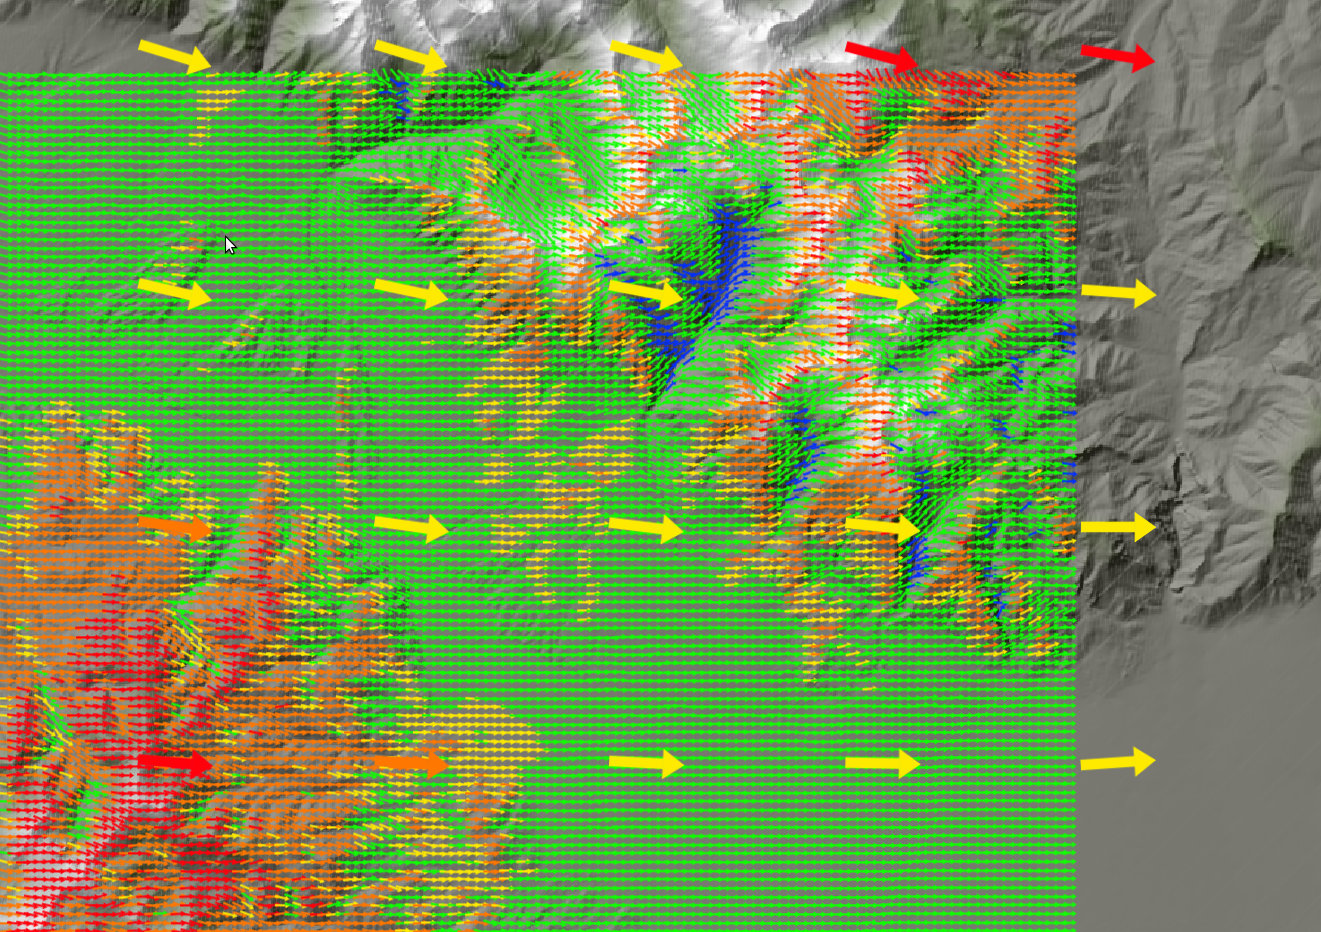
\includegraphics[scale=0.35]							{title_fig}
    \vfill
  	{\Huge
	  7/11/2022 %Date Last Edited
  	}
    \vfill
\end{titlepage}

\section*{Introduction}

Welcome to WindNinja Tutorial 4: Weather Model Initialization.  This tutorial will step you through the process of running a WindNinja simulation that is initialized by output from a weather forecast model.  This tutorial assumes you have already gone through \href{https://weather.firelab.org/windninja/tutorials/WindNinja_tutorial1.pdf}{WindNinja Tutorial 1: The Basics} and \href{https://weather.firelab.org/windninja/tutorials/WindNinja_tutorial2.pdf}{WindNinja Tutorial 2: Diurnal Winds and Non-neutral Stability}, and that you have a working Internet connection.  After this tutorial, you should feel comfortable downloading weather forecast data, using this data to initialize a series of WindNinja runs, and viewing the output.
    
Note:  All required user actions in this tutorial are shown in \textbf{\color{red}red}.

\section*{What is weather model initialization?}

Weather forecasters traditionally use numerical weather models run on large super-computers to help guide forecasts.  These weather models typically simulate large areas (continent scale) and include detailed representations of atmospheric physics such as cloud microphysics, radiant energy transfer, surface fluxes, momentum budgets, and turbulence.  Unfortunately, such detailed representations come with a high computational cost and so these models cannot currently be run operationally at a fine enough resolution to capture local terrain influences.  The typical horizontal resolution of these models is around 4-12 kilometers.  If it is assumed that at least, say, 4 cells are required to resolve flow over a certain terrain feature, then these models can only resolve terrain features that are 16-48 kilometers in size.  And so these models are capable of simulating the larger scale features of weather (fronts, sea-breeze, high and low pressure system movement, etc.) and large scale terrain features (mountain ranges), but do a poor job of capturing fine scale local influences (mechanical terrain modification, slope winds, etc.).

In contrast, WindNinja was developed to simulate fine scale winds (around 100-200 meter resolution) that are dominated by mechanical terrain modification and to a lesser extent diurnal slope winds.  In situations where other factors become important (larger scale processes, sea-breeze, cloud dynamics, etc.) WindNinja's accuracy can severely degrade since it does not explicitly simulate these effects.

The “weather model initialization” feature in WindNinja is an attempt to combine the strengths of traditional coarse weather models and WindNinja into a hybrid model that can better account for the range of scales and physics involved, but at modest computational cost.  The hope is that this will provide more accurate wind forecasts that are relevant to wildland fire managers.

\section*{How does the weather model initialization work?}

The first step in the process is to download the latest forecast (which is automated in WindNinja and described in detail later).  Currently, WindNinja only uses near surface information from the weather forecast model, but the ability to use information at all vertical levels will be added shortly.  The download includes 10 meter wind speed and direction, cloud cover, and 2 meter temperature at the coarse weather model resolution for every output time step.  By default, WindNinja does an individual WindNinja simulation for every output time step of the forecast.  As of version 3.6.0, however, users can select specific time steps from the forecast to simulate. This can save substantial computational time if you have a forecast with many time steps in it, particualry if you are using the conservation of mass and momentum solver. For each WindNinja run, the coarse information is interpolated onto the fine WindNinja grid.  Diurnal winds are then added if the diurnal model is enabled to produce the WindNinja initialized wind field.  Finally, the WindNinja solver is run from this initial wind field to adjust the velocities for the local terrain, stability, and to conserve mass.  The result is a fine resolution forecast of the winds for your area.

\section{Getting Started}

\textbf{\color{red}Start WindNinja by going to Start $\Rightarrow$ Programs $\Rightarrow$ WindNinja \vn\ $\Rightarrow$ WindNinja \vn\ }

\section{Input}
\subsection{Surface Input}

\textbf{\color{red} In the navigation tree, left-click on “Surface Input”.}

\textbf{\color{red} In the input panel, load your existing elevation file or download one using the “Download File” button.}

If you are just practicing, you can use an elevation file provided in the WindNinja installation.  They can be found by going to Start WindNinja by going to Start $\Rightarrow$ Programs $\Rightarrow$ WindNinja \vn\ $\Rightarrow$ etc $\Rightarrow$ windninja $\Rightarrow$ example-files  In the file browser that opens, you will see the elevation file called “missoula\_valley.tif”, and "example\_lcp.lcp". Either of these can be used.

\textbf{\color{red} Select the dominant vegetation type using the “Vegetation” drop down list.  If your elevation file was a FARSITE landscape file, this drop-down box will be grayed out, since the vegetation information is obtained from the landscape file.  In this case, you do not need to select a vegetation type.}

\textbf{\color{red} Select your desired mesh resolution and time zone.}

\subsection{Diurnal Input}

Local diurnal slope winds can optionally be included in a weather model initialization run.  It is normally recommended that diurnal winds be used since it adds more realism to the simulation but only adds a negligible amount of simulation time.

\textbf{\color{red} Left-click on “Diurnal Input” in the navigation tree, then check the “Use Diurnal Wind” check box in the input panel.}

\subsection{Stability Input}

\textbf{\color{red} The stability model can optionally be turned on to simulate an atmosphere that is not necessarily neutral stability.  For this tutorial we will not turn on this model, so leave the “Use Stabililty” check box unchecked.}

\subsection{Wind Input}

\subsubsection{Selecting the weather model and downloading the latest forecast}

\textbf{\color{red} Left-click on “Weather Model” in the navigation tree, which is located under  “Wind Input”.  In the input panel, check the “Weather Model Initialization” check box.}

There are currently 21 different weather forecast model initializations to choose from in WindNinja.  The models are all run by the U.S. National Oceanic and Atmospheric Administration's (NOAA) National Centers for Environmental Prediction (NCEP).  WindNinja accesses these data from two different servers, the NOAA NOMADS server and the University Corporation for Atmospheric Research (UCAR) thredds server.  The two servers provide a means for a fail safe for WindNinja in case one server is down.  We recommend using the NOMADS server as a first choice, as it seems to be more reliable.

The 21 different forecast models have certain advantages and disadvantages depending on your particular situation.  Many of the differences have to do with temporal and spatial resolution and extent, and how often the forecast model is run.  Some of the 21 choices in WindNinja are actually duplicates of the same underlying weather forecast model but provided by both servers.  The table below and following paragraphs give some information about each model.

\begin{landscape}
\begin{longtable}[1]{|p{4.0cm}|p{2.0cm}|p{2.2cm}|p{2.0cm}|p{2.2cm}|p{3.4cm}|p{3.6cm}|}
%\fontsize{8}{12}\selectfont 
%\begin{tabular}{|p{6.6cm}|p{1.3cm}|p{3.3cm}|p{2cm}|p{1.7cm}|p{2.8cm}|p{2.8cm}|}
\hline
\rowcolor{lightgray} Name in WindNinja & Server & Forecast model & Domain & Horizontal resolution & Forecast duration and temporal resolution & Update frequency\\
\hline
UCAR-NDFD-CONUS-2.5-KM & UCAR & National Digitial Forecast Database (NDFD) & contiguous US (CONUS) & 2.5 km & 6 hourly to 168 hrs & 2 per day at 12 and 18 UTC\\
\hline
UCAR-NAM-CONUS-12-KM & UCAR & North American Mesoscale Model (NAM) & contiguous US (CONUS) & 12 km & 3 hourly to 84 hrs & 4 per day at 00, 06, 12, and 18 UTC\\
\hline
UCAR-NAM-ALASKA-11-KM & UCAR & North American Mesoscale Model (NAM) & Alaska & 11 km & 3 hourly to 84 hrs & 4 per day at 00, 06, 12, and 18 UTC\\
\hline
UCAR-RAP-CONUS-13-KM & UCAR & Rapid Refresh Model (RAP) & contiguous US (CONUS) & 13 km & 1 hourly to 18 hrs & updated every 1 hour\\
\hline
UCAR-GFS-GLOBAL-0.5-DEG & UCAR & Global Forecast System (GFS) & global & 0.5 degrees & 3 hourly to 168 hrs & 4 per day at 00, 06, 12, and 18 UTC\\
\hline
NOMADS-GFS-GLOBAL-0.25-DEG & NOMADS & Global Forecast System (GFS) & global & 0.25 degrees & 1 hourly to 120 hrs 3 hourly for days 5-16 & 4 per day at 00, 06, 12, and 18 UTC\\
\hline
NOMADS-HIRES-ARW-ALASKA-5-KM & NOMADS & High Resolution WRF - ARW Core & Alaska & 5 km & 1 hourly to 48 hrs & 1 per day at 06 UTC\\
\hline
NOMADS-HIRES-FV3-ALASKA-5-KM & NOMADS & High Resolution WRF - FV3 Core & Alaska & 5 km & 1 hourly to 48 hrs & 1 per day at 06 UTC\\
\hline
NOMADS-HIRES-ARW-CONUS-5-KM & NOMADS & High Resolution WRF - ARW Core & contiguous US (CONUS) & 5 km & 1 hourly to 48 hrs & 2 per day at 00 and 12 UTC\\
\hline
NOMADS-HIRES-FV3-CONUS-5-KM & NOMADS & High Resolution WRF - FV3 Core & contiguous US (CONUS) & 5 km & 1 hourly to 48 hrs & 2 per day at 00 and 12 UTC\\
\hline
NOMADS-HIRES-GUAM-5-KM & NOMADS & High Resolution WRF - ARW Core & Guam & 5 km & 1 hourly to 48 hrs & 4 per day at 00, 06, 12 and 18 UTC\\
\hline
NOMADS-HIRES-HAWAII-5-KM & NOMADS & High Resolution WRF - ARW Core & Hawaii & 5 km & 1 hourly to 48 hrs & 4 per day at 00, 06, 12 and 18 UTC\\
\hline
NOMADS-HIRES-PUERTO-RICO-5-KM & NOMADS & High Resolution WRF - ARW Core & Puerto Rico & 5 km & 1 hourly to 48 hrs & 4 per day at 00, 06, 12 and 18 UTC\\
\hline
NOMADS-NAM-ALASKA-11.25-KM & NOMADS & North American Mesoscale Model (NAM) & Alaska & 11.25 km & 3 hourly to 36 hrs 6 hourly to 86 hrs & 4 per day at 00, 06, 12 and 18 UTC\\
\hline
NOMADS-NAM-CONUS-12-KM & NOMADS & North American Mesoscale Model (NAM) & contiguous US (CONUS) & 12 km & 1 hourly to 36 hrs 3 hourly to 86 hrs & 4 per day at 00, 06, 12 and 18 UTC\\
\hline
NOMADS-NAM-NEST-CONUS-3-KM & NOMADS & North American Mesoscale Model (NAM) & contiguous US (CONUS) & 3 km & 1 hourly to 60 hrs & 4 per day at 00, 06, 12 and 18 UTC\\
\hline
NOMADS-NAM-NEST-ALASKA-3-KM & NOMADS & North American Mesoscale Model (NAM) & contiguous US (CONUS) & 3 km & 1 hourly to 60 hrs & 4 per day at 00, 06, 12 and 18 UTC\\
\hline
NOMADS-NAM-NEST-HAWAII-3-KM & NOMADS & North American Mesoscale Model (NAM) & Hawaii & 3 km & 1 hourly to 60 hrs & 4 per day at 00, 06, 12 and 18 UTC\\
\hline
NOMADS-NAM-NEST-PUERTO-RICO-3-KM & NOMADS & North American Mesoscale Model (NAM) & Puerto Rico & 3 km & 1 hourly to 60 hrs & 4 per day at 00, 06, 12 and 18 UTC\\
\hline
NOMADS-NAM-NORTH-AMERICA-32-KM & NOMADS & North American Mesoscale Model (NAM) & North America & 32 km & 3 hourly to 36 hrs 6 hourly to 86 hrs & 4 per day at 00, 06, 12 and 18 UTC\\
\hline
NOMADS-HRRR-CONUS-3-KM & NOMADS & High Resolution Rapid Refresh (HRRR) & contiguous US (CONUS) & 3 km & 1 hourly to 18 hrs & updated every 1 hour\\
\hline
NOMADS-HRRR-ALASKA-3-KM & NOMADS & High Resolution Rapid Refresh (HRRR) & Alaska & 3 km & 1 hourly to 18 hrs & updated every 1 hour\\
\hline
NOMADS-HRRR-CONUS-SUBHOURLY-3-KM & NOMADS & High Resolution Rapid Refresh (HRRR) & contiguous US (CONUS) & 3 km & every 15 min to 18 hrs & updated every 1 hour\\
\hline
NOMADS-HRRR-ALASKA-SUBHOURLY-3-KM & NOMADS & High Resolution Rapid Refresh (HRRR) & Alaska & 3 km & every 15 min to 18 hrs & updated every 1 hour\\
\hline
NOMADS-RAP-CONUS-13-KM & NOMADS & Rapid Refresh (RAP) & contiguous US (CONUS) & 13 km & 1 hourly to 18 hrs & updated every 1 hour\\
\hline
NOMADS-RAP-NORTH-AMERICA-32-KM & NOMADS & Rapid Refresh (RAP) & North America & 32 km & 1 hourly to 18 hrs & updated every 1 hour\\
\hline
%\end{tabular}
\caption{Comparison of the forecast weather models available in WindNinja.}
\end{longtable}
\end{landscape}

Users should choose a model that best fits their particular situation, keeping in mind that there may be several forecast models that fit.  In these situations, it isn't a bad idea to try several of them and examine the differences in the results.


Below is some general information to consider when choosing a forecast model:
\begin{itemize}
\item Higher spatial resolution is generally better than lower resolution.
\item Since forecast accuracy degrades with time, forecast models that are run more often might give more accurate results.  An example of this degradation is shown in Figure 2.1.  The reason for degradation with time is that small errors in the model can accumulate over time.  So if a forecast for 1 hour from now was simulated 11 hours ago, that forecast will probably be less accurate than one that was simulated 1 hour ago.  The more recent forecast would start with a better description of the current state of the atmosphere and the small accumulating errors wouldn't have as much time to grow.
\end{itemize}


\begin{figure}[H]
	\centering
	\label{ndfd_degrade}
	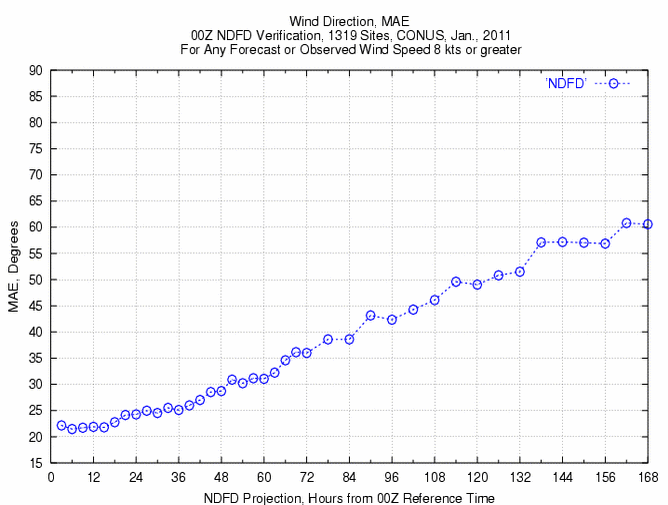
\includegraphics[scale=0.75]{degrade_w_time}
	\caption*{An example showing how a forecast can degrade with time.  This graph compares wind direction forecast by NDFD in Jan. 2011 with measurements from across the U.S.  The time (in hours) since the forecast was issued is shown on the x-axis, and the mean absolute error (MAE) of predicted wind direction is shown on the y-axis.}
\end{figure}

\begin{itemize}
\item The forecast model must cover your modeling area.  Each forecast model has a limited area, and if you try to use a forecast model for an elevation file that is outside the forecast area, WindNinja will report an error.  Images of some of the weather model domains are shown below to give you an idea of what areas the models might cover.
\end{itemize}

\begin{figure}[H]
	\centering
	\label{UCAR_NDFD_Domain}
	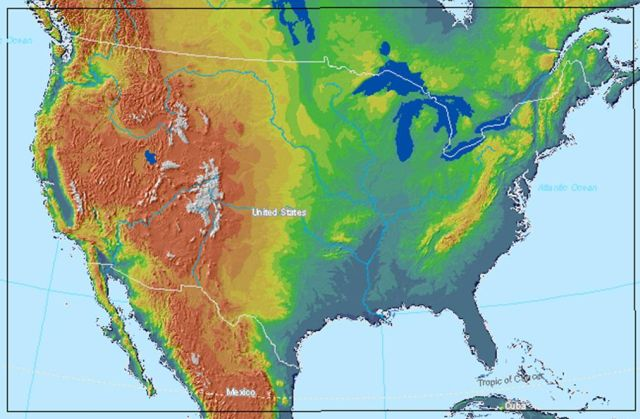
\includegraphics[scale=1.0]{NDFD_domain}
	\caption*{UCAR-NDFD-CONUS-2.5-km domain.}
\end{figure}
\begin{figure}[H]
	\centering
	\label{UCAR_NDFD_Domain}
	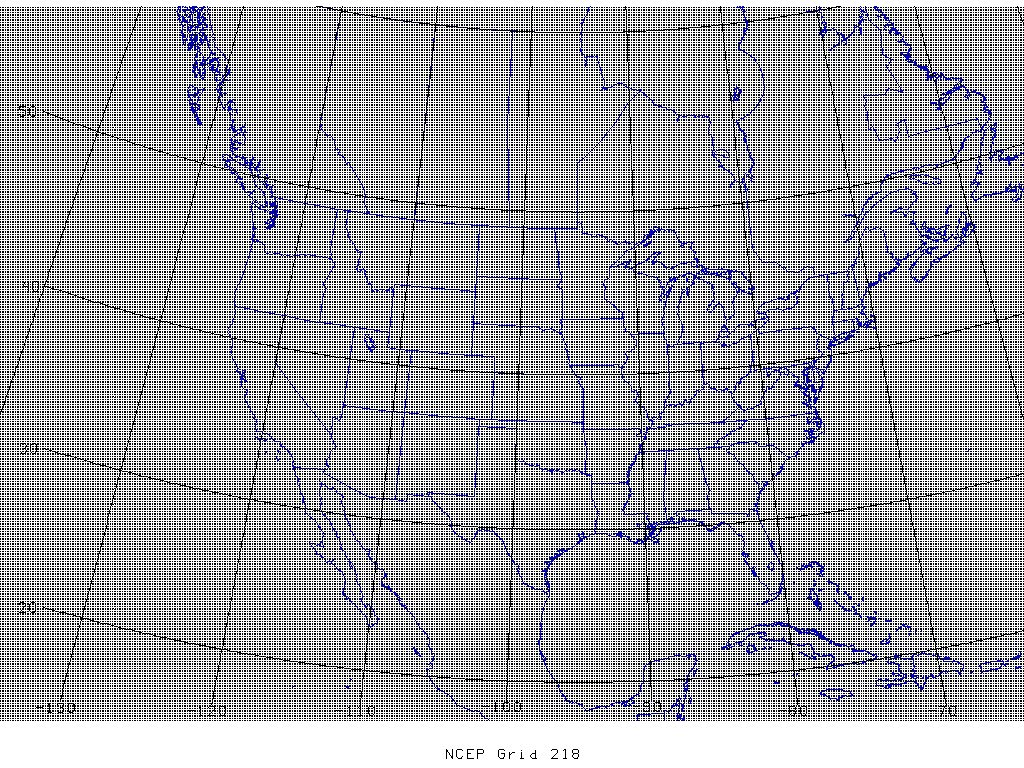
\includegraphics[scale=0.30]{NAM_1}
	\caption*{UCAR-NAM-CONUS-12km domain.}
\end{figure}
\begin{figure}[H]
	\centering
	\label{RAP_CONUS}
	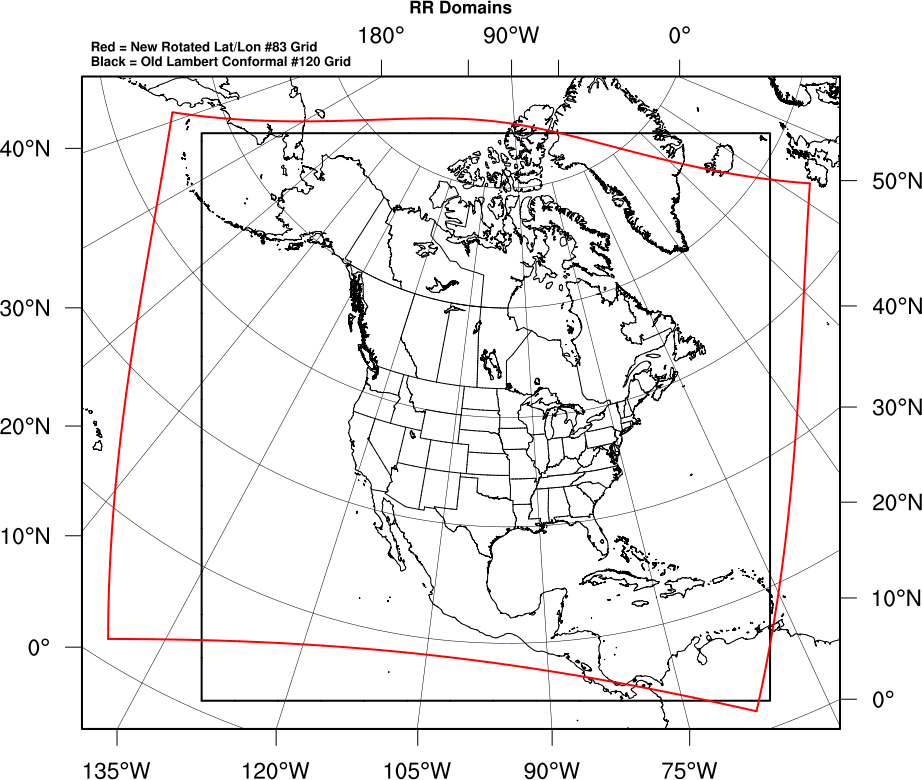
\includegraphics[scale=0.35]{UCAR_RAP_domain}
	\caption*{UCAR-RAP-CONUS-13km domain.}
\end{figure}
\begin{figure}[H]
	\centering
	\label{RAP_CONUS}
	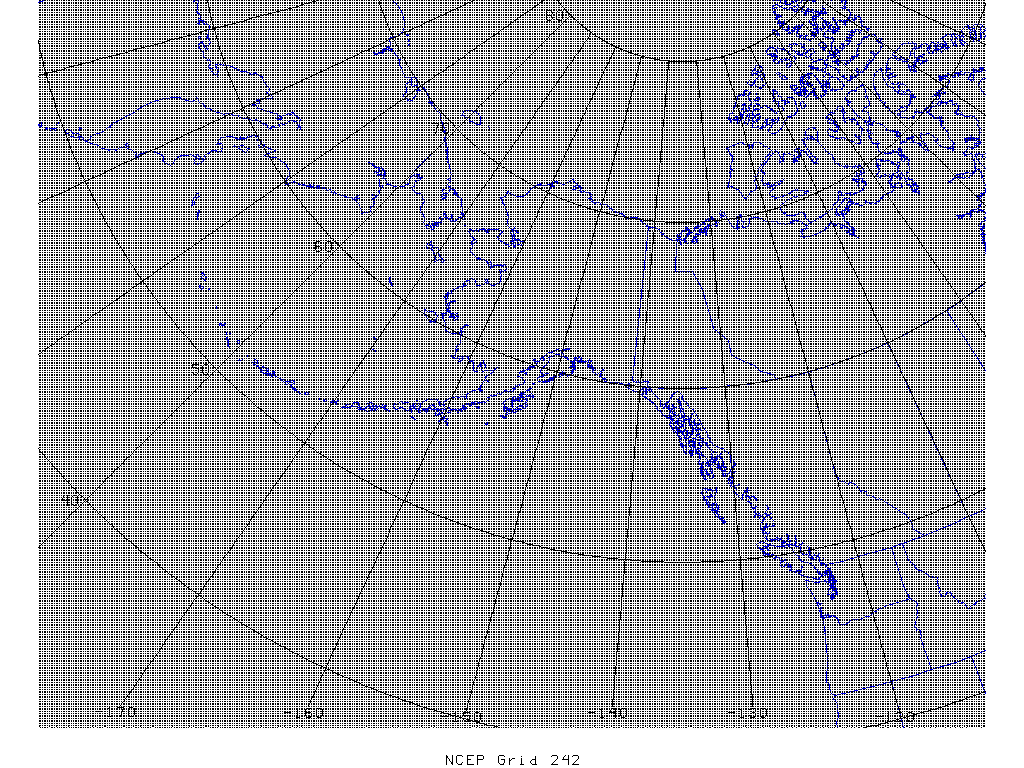
\includegraphics[scale=0.30]{NAM_2}
	\caption*{UCAR-NAM-Alaska-11km domain.}
\end{figure}
Some comments about each forecast model:
\begin{itemize}
\item \textbf{NDFD} – This model has good spatial resolution (2.5 km), but currently only 6 hour temporal resolution.  It provides a relatively long forecast (7 days).  Unlike the other models, this one is not just “raw” forecast model output.  The UCAR-NDFD-CONUS-2.5-KM starts out as “raw” output from a computer model, but goes through a process of inspection and manipulation by local weather forecasters.  The hope is that the expertise of the local weather forecasters can add value to the forecast.  At this time, it is unclear if this method is an advantage or disadvantage for use in WindNinja, as certain issues may arise such as “border” effects where one forecaster's area meets another.

\item \textbf{NAM} – This model is a good all-round choice, providing a forecast out to 3.5 days and covering all of North America.  The NAM model is one of the most commonly used mesoscale models in the U.S.

\item \textbf{HRRR} and \textbf{NAM-NEST} – The HRRR and the NAM-NEST models have the highest resolution of all the models (3 km), excluding NDFD. This high resolution allows these models to resolve some smaller atmospheric features better than other models (sea-breezes, local density-driven winds, etc.). These models also produce the highest temporal output resolution (every hour). The HRRR is specifically designed for very short range forecasts (out to 18 hours). The NAM-NEST models produce forecasts out to 60 hours. The HRRR uses advanced data assimilation (e.g., for lightning) and explicit simulation of convection, which should translate to better thunderstorm predictions. Another big advantage of the HRRR over most of the other models is that it is run every hour, so that its forecasts use very current information about the state of the atmosphere.  The HRRR would likely be the best model to use if you need a very short term forecast (say, for the next few hours).

\item \textbf{RAP} – This model is very similar to HRRR, except at a coarser resolution.  Probably only use this model if HRRR is not possible.

\item \textbf{GFS} – This model has global coverage and so is available anywhere in the world.  It is relatively coarse at 0.25 degrees.  It is the only global coverage model available.  In general, users simulating areas outside North America must use this model.  The model also has the longest forecast duration (out to 16 days), although it is questionable whether winds can be predicted with any amount of accuracy this far out.
\end{itemize}

WindNinja has an automated system to make downloading the latest forecasts very easy.  Essentially, the user just needs to choose the forecast model and number of hours they want and left-click the “Download data” button.  The number of hours you enter is the number of hours since the weather model forecast was run (which depends on the model, and would be anywhere from 1 to 24 hours ago).  Behind-the-scenes what happens is: WindNinja knows the area you want to simulate based on your elevation file, and so a message is sent over your Internet connection to a web service on the NOMADS or UCAR server asking for the forecast data for an area slightly bigger than your elevation file domain.  The web server clips this area out of the full forecast data coverage, and sends it to your computer.

\textbf{\color{red} In the input panel for weather model initialization, select the weather model you want to download using the “Download Weather Data” drop-down box.  Enter the number of forecast hours that you want.  Click the “Download data” button to download the forecast.}

The download of the file should normally only take a few seconds, but will depend on your Internet connection speed, spatial extent of your elevation file, number of forecast hours, and forecast model selected.  WindNinja builds a directory structure (folders) starting where your elevation file is located to make it easier for you (and WindNinja) to keep track of the forecast and output files made by WindNinja during a weather model initialization run.  It is not recommended to manually move, rename, or delete these files until after you are done with your simulations and have closed out of WindNinja.

When your download is finished, a new folder will appear in the “Downloaded forecasts” list on the input panel.  You can download several forecasts (selecting different forecast models) at this time and each will be added to the list.

The “Downloaded forecasts” list is an expandable tree structure showing the files and folders that WindNinja has made during the download process.  You can expand the folders to navigate down to the actual downloaded weather file, which has a “.nc” file extension (which stands for “NetCDF”, a standard weather file type) for the UCAR server or a “.zip” file extension for the NOMADS server (the zip contains many GRIB files, which is a common weather raster data format).  The naming convention used for these folders and files is automatically generated by WindNinja using the forecast model name, forecast start time, and elevation filename.  At the top level, there is a folder for each type of forecast model for your elevation file that looks like this:

\begin{figure}[H]
	\centering
	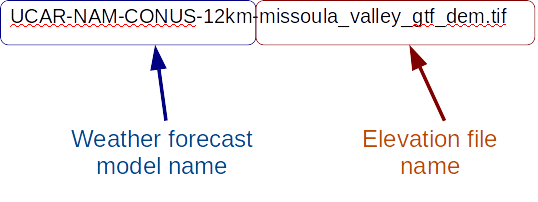
\includegraphics[scale=1.0]{fil_diag}
\end{figure}

Note:  This is a \textbf{folder}, even though it has the “.tif” at the end.

Under this folder, there is a folder for each time you've downloaded a forecast for this model and elevation file (for example, if you downloaded a forecast yesterday and then downloaded a forecast today, 2 folders would be shown, one with yesterday's date/time and one with today's date/time).  The date/time used for the folder name is the date and time of the first time “step” in the forecast.  WindNinja calls this the “first forecast time” and it is used to identify when the forecast model was run by the weather model provider.  If you download a forecast, and then download the same forecast again before a new forecast has been issued (essentially downloading the exact same forecast twice), the second forecast downloaded will just replace the first forecast and so only one folder will be made.

The date/time naming format for these folders is shown below with colors added for clarity.  Unfortunately, these dates and times are in Coordinated Universal Time (UTC), not local time.  Conversion to local time is described later in this tutorial.

\begin{figure}[H]
	\centering
	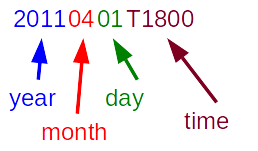
\includegraphics[scale=1.0]{UTC_diag}
\end{figure}

Inside of these date/time folders is where the downloaded forecast file is located, and is also where all of WindNinja's output files will be written to.  The forecast file is labeled using the same date/time scheme as above, and has the “.nc” or “.zip” file extension added.


\textbf{You can also use the NetCDF output from a WRF-ARW custom simulation}. This feature is useful for researchers running custom WRF simulations. Note that the WRF output file must be a NetCDF “wrfout” file with a “.nc” file extension. To use a custom wrfout file, simply put the wrfout file in the same directory as your DEM and WindNinja will auto-detect it and make it selectable in the “Downloaded forecasts” list.

Since you may have many different forecasts downloaded to your computer, you need to tell WindNinja which one to use.  This is done by simply selecting (left-click) the forecast file in the “Downloaded forecasts” list.  \textbf{Be sure that you select the “.nc” or “.zip” forecast file and \underline{not a folder}.}

\textbf{\color{red}Select the desired forecast file in the “Downloaded forecasts” list by left-clicking.}

After you select your forecast file, the local time for the “first forecast time” appears below the “Downloaded forecasts” list area.  This local time uses the time zone you specified earlier.

By default WindNinja will simulate each time step in the weather model forecast. As of version 3.6.0, however, you can choose to select specific time steps from the forecast to simulate. To do this, check the box labeled “Select specific time steps" located below the “Download forecasts" box. This will activate the window below the “Select specific time steps" making the list of time steps selectable. Initially, all time steps will be selected (selected time steps are highlighted in grey). You can click on specific time steps to de-select or choose the “Select None" button below the window to de-select all time steps and then click on time steps to select the ones you want to simulate.

\section{Output}
The same output files are written for weather model initialized simulations as other simulations (Google Earth, Fire Behavior, Shape files).  WindNinja does a separate simulation for each weather forecast model time “step” and writes output files for each of these time “steps”.  There is also an optional choice of writing output for the “raw” weather forecast model data, which is written at that forecast model's resolution.  All of these output files are written to the date/time folder described above.  The naming convention for the WindNinja output files is similar to a “Domain Average Wind” initialized simulation with diurnal turned on.  You should reference \href{https://weather.firelab.org/windninja/tutorials/WindNinja_tutorial2.pdf}{WindNinja Tutorial 2: Diurnal Winds and Non-neutral Stability} for more information.  The “raw” weather forecast output files are written with a similar naming convention, except that in place of the elevation file name is the weather forecast model name and the resolution is absent (since the resolution is that of the forecast model).  Below is an example of a Google Earth output file name and the corresponding “raw” forecast model file name for April 11th at 1500.  The elevation file used was called “missoula\_valley.tif” and the weather forecast model was the “UCAR-NAM-CONUS-12-KM”.

missoula\_valley\_04-11-2011\_1500\_176m.kmz $\Leftarrow$ WindNinja output file

UCAR-NAM-CONUS-12-KM-04-11-2011\_1500.kmz  $\Leftarrow$  “raw” forecast file

\textbf{\color{red} In the navigation tree, left-click on “Output” and select the “Output Height”, “Output Speed Units”, and“Clip output by:” values you want.  Also, check the “Write Raw Weather Model Output” checkbox.}

Another feature in WindNinja is the ability to write out a FARSITE atmosphere file (*.atm).  This might be useful if you are planning on using your WindNinja simulation in a FARSITE fire spread simulation.  The atmosphere file is used in FARSITE to define which WindNinja files should be used during the fire simulation.  Since FARSITE uses WindNinja's fire behavior files (*.asc), this atmosphere option is only available if you are writing fire behavior files.  This option can be enabled in WindNinja on the Output$\Rightarrow$Fire Behavior input panel.

\textbf{\color{red}Choose the types of output files you would like by left-clicking the type in the navigation tree and filling out the corresponding input panel.}

Note that the fire behavior cloud cover file written by WindNinja uses the gridded cloud cover provided by the weather forecast model.

\section{Solve}

\textbf{\color{red} Left-click on “Solve” in the navigation tree.  Set the number of processors you would like using the “Number of Processors” text box.  Finally, left-click the “Solve” button to start the simulation(s).}

Since WindNinja is doing a simulation for each weather forecast model time “step”, it may take a while for WindNinja to complete the simulations.  Typical simulation time for an average dual core computer in 2020 should be around 1-5 minutes depending on the computer, number of forecast model time “steps”, simulation resolution, etc.

\textbf{\color{red} When the simulation is finished, close the progress window.}

A handy feature in WindNinja is the “Open Output Files Path” button on the Solve page.  If you click this, it will open the folder where all of the output files for the last run were written to.

This concludes \textbf{WindNinja Tutorial 4: Weather Model Initialization}.

\end{document}
